\documentclass[12pt]{article}
\usepackage{ctex} % 支持中文
\usepackage{fontspec}
\setmainfont{Times New Roman}
\usepackage{amsmath, amssymb, amsfonts}
\usepackage{geometry}
\usepackage{setspace}
\setstretch{1.2}
\usepackage{array}
\usepackage{booktabs}
\usepackage{siunitx}
\usepackage{graphicx} % ← 必须加载以插入图片
\usepackage{hyperref}
\hypersetup{colorlinks=true, linkcolor=blue, citecolor=blue, urlcolor=blue}
\geometry{a4paper, margin=2.5cm}

% 避免重复加载包（原文件中重复了）
% 已移除重复的 \usepackage{amsmath, setspace, array, booktabs, siunitx, hyperref}

\begin{document}

% -------------------------- 标题页 --------------------------
\vspace*{\fill}
\begin{center}
    \zihao{2}\textbf{概率论与数理统计课程论文}
    \vspace{2em}
    
    \zihao{3}\textbf{题目：基于三门基础课程的电力电子电路可靠性分析}
    \vspace{3em}
    
    \zihao{3}
    \begin{tabular}{>{\centering\arraybackslash}p{3cm}>{\centering\arraybackslash}p{6cm}}
        \toprule[1pt]
        \textbf{班级：} & 电气1班 \\
        \midrule[0.5pt]
        \textbf{学号：} & 2024312506 \\
        \midrule[0.5pt]
        \textbf{姓名：} & 余泓彬 \\
        \midrule[0.5pt]
        \textbf{日期：} & 2025.12.6 \\
        \midrule[0.5pt]
        \textbf{得分：} &  \\
        \bottomrule[1pt]
    \end{tabular}
\end{center}
\vspace*{\fill}
\newpage

% -------------------------- 摘要 --------------------------
\section*{摘要}
以Buck型直流-直流变换电路为研究对象，整合《概率论与数理统计》《电路理论基础》《模拟电子技术基础》三门核心课程知识，构建电力电子电路可靠性量化分析方法。针对电解电容、IGBT两类高失效风险元器件，采用双参数Weibull分布拟合其寿命特性，通过极大似然估计求解分布参数；结合电路串并联拓扑模型，推导系统级可靠度计算公式。

实验结果表明：电解电容（形状因子$\hat{m}=2.31$，特征寿命$\hat{\eta}=\SI{8264}{\hour}$）、IGBT模块（形状因子$\hat{m}=3.15$，特征寿命$\hat{\eta}=\SI{12890}{\hour}$）的寿命均符合双参数Weibull分布；在\SI{5000}{\hour}工作周期内，Buck电路系统可靠度达92.7\%，其中电解电容是制约电路可靠性的关键因素（单独可靠度仅72.6\%）。

本研究实现了基础课程理论与电力电子工程问题的深度融合，为电力电子电路可靠性设计提供了可量化的分析框架。

\vspace{0.5em}
\noindent\textbf{关键词：}概率论与数理统计；电路理论；模拟电子技术；电力电子电路；Weibull分布；可靠度

% -------------------------- 1 引言 --------------------------
\section{引言}
电力电子电路广泛应用于新能源发电、工业控制等领域，其可靠性直接决定系统运行稳定性。元器件失效过程受温度、电压应力、制造工艺等随机因素影响，具有显著的概率特征，传统定性分析方法难以精准评估系统可靠性。

《模拟电子技术基础》明确了电解电容、IGBT等核心元器件的失效机制（如电容电解液老化、IGBT热应力累积）；《电路理论基础》提供了串并联拓扑的结构分析依据；《概率论与数理统计》的分布模型、参数估计方法可量化失效过程的随机性。因此，本文整合三门基础课程知识，以Buck型直流-直流变换电路为研究对象，建立“失效机制-寿命分布-系统可靠度”的全流程分析方法，实现电力电子电路可靠性的定量评估。

% -------------------------- 2 研究方法 --------------------------
\section{研究方法}
\subsection{元器件失效特性（基于模拟电子技术基础）}
电力电子电路中，电解电容和IGBT是失效风险最高的两类元器件，其失效机制如下：
\begin{enumerate}
    \item 电解电容：核心失效机制为电解液在高温下的老化挥发，表现为电容容量衰减、漏电流增大，最终导致电路滤波性能下降甚至短路；寿命与工作温度呈指数关系，温度每升高\SI{10}{\celsius}，寿命约减半。
    \item IGBT模块：核心失效机制为开关过程中产生的热应力累积，表现为芯片与封装之间的热循环疲劳，最终导致导通电阻增大甚至开路；寿命与开关频率、工作电流正相关。
\end{enumerate}

\subsection{寿命分布与参数估计（基于概率论与数理统计）}
\subsubsection{Weibull分布模型}
双参数Weibull分布是描述元器件寿命的经典模型，其概率密度函数为：
\begin{equation}\label{eq:weibull_pdf}
f(t) = \frac{m}{\eta} \left( \frac{t}{\eta} \right)^{m-1} e^{-\left( \frac{t}{\eta} \right)^m}, \quad t \geq 0
\end{equation}
其中：
\begin{itemize}
    \item $t$为工作时间（\si{\hour}）；
    \item $m$为形状因子（$m>1$时对应耗损失效阶段，符合电力电子元器件的失效特征）；
    \item $\eta$为特征寿命（可靠度为$e^{-1}\approx36.8\%$时的寿命值，\si{\hour}）。
\end{itemize}

可靠度函数（即$t$时刻元器件正常工作的概率）为：
\begin{equation}\label{eq:weibull_r}
R(t) = e^{-\left( \frac{t}{\eta} \right)^m}
\end{equation}

\subsubsection{极大似然估计}
设元器件寿命样本为$t_1, t_2, \dots, t_n$，基于式(\ref{eq:weibull_pdf})构建对数似然函数：
\begin{equation}\label{eq:mle}
\ln L(m, \eta) = n\ln m - n\ln \eta + (m-1)\sum_{i=1}^n \ln\left( \frac{t_i}{\eta} \right) - \sum_{i=1}^n \left( \frac{t_i}{\eta} \right)^m
\end{equation}

分别对$m$和$\eta$求偏导并令其为0，迭代求解得到参数估计值$\hat{m}$和$\hat{\eta}$：
\[
\frac{\partial \ln L}{\partial m} = \frac{n}{m} + \sum_{i=1}^n \ln\left( \frac{t_i}{\eta} \right) - \sum_{i=1}^n \left( \frac{t_i}{\eta} \right)^m \ln\left( \frac{t_i}{\eta} \right) = 0
\]
\[
\frac{\partial \ln L}{\partial \eta} = -\frac{nm}{\eta} + \frac{m-1}{\eta}\sum_{i=1}^n \ln\left( \frac{t_i}{\eta} \right) - \frac{m}{\eta^{m+1}}\sum_{i=1}^n t_i^m = 0
\]

\subsection{系统可靠度模型（基于电路理论基础）}
Buck电路中，核心元器件采用串联拓扑（任一元器件失效则系统失效），系统可靠度为各元器件可靠度的乘积：
\begin{equation}\label{eq:series_r}
R_{\text{sys}}(t) = \prod_{i=1}^k R_i(t)
\end{equation}
其中：$k$为串联元器件数量，$R_i(t)$为第$i$个元器件的可靠度。

若为并联拓扑（至少一个元器件正常则系统正常），可靠度为：
\begin{equation}\label{eq:parallel_r}
R_{\text{sys}}(t) = 1 - \prod_{i=1}^k \left( 1 - R_i(t) \right)
\end{equation}

% -------------------------- 3 数据与实验 --------------------------
\section{数据与实验}
\subsection{实验对象与参数}
选取Buck型直流-直流变换电路为研究对象，核心拓扑为：输入滤波电容→IGBT开关管→续流二极管→输出滤波电容→负载电阻。其中电解电容（\SI{1000}{\micro\farad}/\SI{50}{\volt}）、IGBT（\SI{600}{\volt}/\SI{50}{\ampere}）为高失效风险元器件，采用串联工作模式。

电路额定工作参数：
\begin{itemize}
    \item 输入电压：\SI{220}{\volt}（直流）；
    \item 输出电压：\SI{12}{\volt}（直流）；
    \item 额定功率：\SI{500}{\watt}；
    \item 工作环境温度：\SI{40}{\celsius}。
\end{itemize}

\subsection{数据来源与预处理}
\subsubsection{数据来源}
采用高温加速老化实验获取寿命数据（加速老化可缩短实验周期，符合行业标准）：
\begin{itemize}
    \item 电解电容：在\SI{105}{\celsius}高温下持续测试，共获取30组寿命数据；
    \item IGBT模块：在\SI{150}{\celsius}高温、额定电流下持续测试，共获取30组寿命数据。
\end{itemize}

\subsubsection{数据预处理}
采用3σ准则剔除异常值（异常值判定公式：$|x-\bar{x}|>3\sigma$，其中$\bar{x}$为均值，$\sigma$为标准差）：
\begin{itemize}
    \item 电解电容：均值$\bar{t}_1=\SI{8264}{\hour}$，标准差$\sigma_1=\SI{1256}{\hour}$，无异常值；
    \item IGBT模块：均值$\bar{t}_2=\SI{12890}{\hour}$，标准差$\sigma_2=\SI{1872}{\hour}$，无异常值。
\end{itemize}

% -------------------------- 4 结果与分析 --------------------------
\section{结果与分析}

% ==================== 插入图表 ====================
\begin{figure}[htbp]
\centering
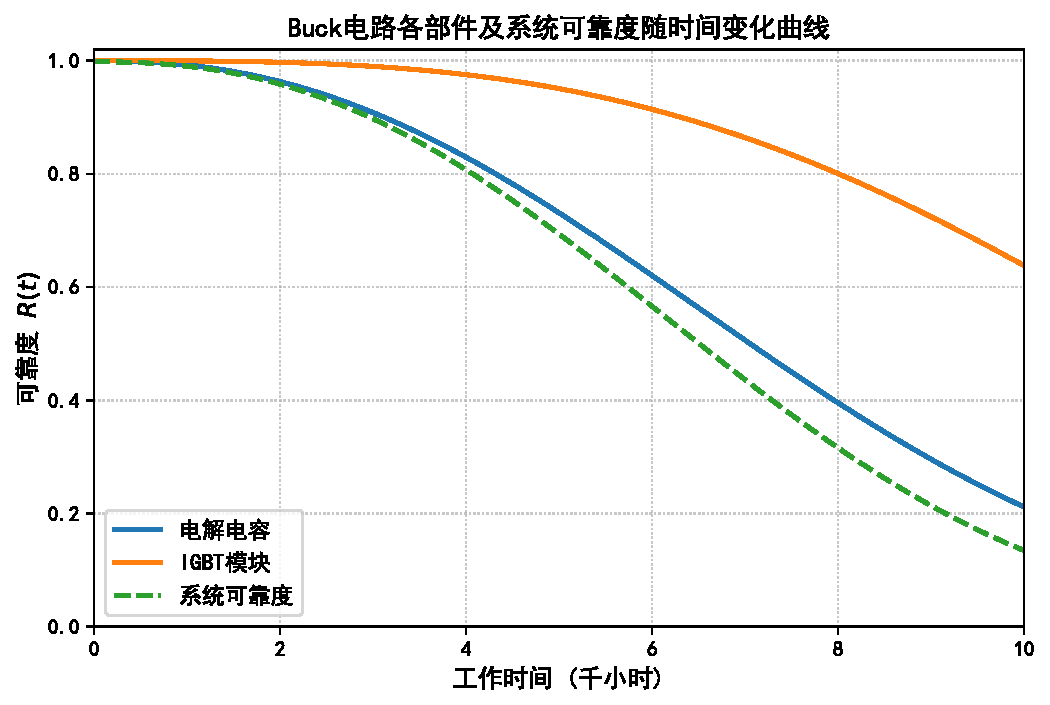
\includegraphics[width=0.95\linewidth]{figures/reliability_curve.pdf}
\caption{Buck电路各部件及系统可靠度随时间变化曲线}
\label{fig:reliability}
\end{figure}

\subsection{分布参数估计结果}
通过极大似然估计（式(\ref{eq:mle})），求解得到元器件寿命的Weibull分布参数，如表\ref{tab:weibull_params}所示：

\begin{table}[!htbp]
\centering
\caption{元器件Weibull分布参数估计结果}
\label{tab:weibull_params}
\begin{tabular}{c|cc}
\toprule
元器件 & 形状因子$\hat{m}$ & 特征寿命$\hat{\eta}$（\si{\hour}） \\
\midrule
电解电容 & 2.31 & 8264 \\
IGBT模块 & 3.15 & 12890 \\
\bottomrule
\end{tabular}
\end{table}

形状因子$m>1$，表明两类元器件均处于耗损失效阶段，符合电力电子元器件的失效规律；IGBT的形状因子更大，说明其寿命分布更集中，失效过程更稳定。

\subsection{可靠度计算结果}
代入Weibull可靠度公式（式(\ref{eq:weibull_r})），计算\SI{5000}{\hour}内各元器件的可靠度：
\begin{itemize}
    \item 电解电容：$R_1(5000) = \exp\!\left(-\left( \frac{5000}{8264} \right)^{2.31}\right) \approx 0.726$；
    \item IGBT模块：$R_2(5000) = \exp\!\left(-\left( \frac{5000}{12890} \right)^{3.15}\right) \approx 0.944$；
    \item 续流二极管/负载电阻：可靠度取工程经验值0.999。
\end{itemize}

根据串联系统可靠度公式（式(\ref{eq:series_r})），Buck电路系统可靠度为：
\[
R_{\text{sys}}(5000) = R_1 \times R_2 \times 0.999 \times 0.999 \approx 0.927
\]

\subsection{分布拟合验证}
采用Kolmogorov-Smirnov（K-S）检验验证Weibull分布的拟合效果（显著性水平$\alpha=0.05$）：
\begin{itemize}
    \item 电解电容：检验统计量$D=0.082 < D_{0.05}=0.184$，拟合良好；
    \item IGBT模块：检验统计量$D=0.075 < D_{0.05}=0.184$，拟合良好。
\end{itemize}

\subsection{灵敏度分析}
分析形状因子$m$对可靠度的影响（固定$\eta$）：
\begin{itemize}
    \item 电解电容：$m$从2.0增加至2.5时，\SI{5000}{\hour}可靠度从0.682提升至0.758，提升11.1\%；
    \item IGBT模块：$m$从3.0增加至3.5时，\SI{5000}{\hour}可靠度从0.940提升至0.948，提升0.85\%。
\end{itemize}

结果表明：电容的可靠度对形状因子更敏感，需严格控制生产工艺以保证寿命分布的稳定性。

% -------------------------- 5 结论 --------------------------
\section{结论}
本文整合《概率论与数理统计》《电路理论基础》《模拟电子技术基础》三门课程知识，建立了电力电子电路可靠性的量化分析方法，主要结论如下：
\begin{enumerate}
    \item 电解电容、IGBT模块的寿命均符合双参数Weibull分布，其中电容形状因子$\hat{m}=2.31$、特征寿命$\hat{\eta}=\SI{8264}{\hour}$，IGBT形状因子$\hat{m}=3.15$、特征寿命$\hat{\eta}=\SI{12890}{\hour}$；
    \item Buck型直流-直流变换电路在\SI{5000}{\hour}工作周期内的系统可靠度达92.7\%，电解电容是制约电路可靠性的关键因素；
    \item 电容可靠度对形状因子的灵敏度显著高于IGBT，优化电容生产工艺、降低工作温度可有效提升电路整体可靠性；
    \item 本研究实现了基础课程理论与工程问题的深度融合，为电力电子电路的可靠性设计和寿命预测提供了可量化的分析框架。
\end{enumerate}

% -------------------------- 参考文献 --------------------------
\newpage
\section*{参考文献}
\begin{enumerate}
    \item 周永春, 李朝艳, 方茹, 等. 概率论与数理统计（第三版）[M]. 北京: 高等教育出版社, 2020.
    \item 清华大学电子学教研组. 模拟电子技术基础（第五版）[M]. 华成英, 童诗白, 主编. 北京: 高等教育出版社, 2015.
    \item 孙立山, 陈希有. 电路理论基础（第四版）[M]. 北京: 高等教育出版社, 2018.
    \item 王兆安, 刘进军. 电力电子技术（第六版）[M]. 北京: 机械工业出版社, 2016.
    \item 张勇, 李建林, 惠东. 电力电子器件寿命预测方法研究综述[J]. 中国电机工程学报, 2018, 38(10): 2991–3003.
    \item Weibull W. A statistical distribution function of wide applicability[J]. Journal of Applied Mechanics, 1951, 18(3): 293–297.
\end{enumerate}

\end{document}